\documentclass[12pt]{article}
\usepackage[english]{babel}
\usepackage{amsmath,amsthm}
\usepackage{graphicx}
\usepackage{caption}
\usepackage{subcaption}
\usepackage{graphicx}
\usepackage{amsfonts}
\usepackage{float}
\usepackage{indentfirst}
\usepackage{lscape}
\usepackage[top=2.5cm,bottom=2.5cm,right=2.5cm,left=2.5cm]{geometry}
\usepackage{titlesec}
\setcounter{secnumdepth}{5}

% ----------------------------------------------------------------
\begin{document}

\section{Color Constrast Occurence}

Here we will see the different steps that we have to follow to compute the C$_2$O descriptor. There will be three main steps that we will have to study, The transformation through a perceptual space, the computation of the coocurence matrix and the computation of the signature vector.

\subsection{Transformation through a perceptual space}

First of all, we need to pass our image in the L$^*$a$^*$b$^*$ space to get directly a representation of it in a space which split the luminance and the chromatic information.

For doing that, we first need to pass the image in the XYZ space and choose the correct standard illuminant A.
\vspace{0.5cm}
$$A=\begin{pmatrix}
	X_r&X_g&X_b\\
	Y_r&Y_g&Y_b\\
    Z_r&Z_g&Z_b
\end{pmatrix}$$


That parameter depends on the characteristics of the device used to take the picture: it represents how the device interpret the real colors. In our case, there are many different devices that have been used to take the different pictures so we will have to make a choice. Some standard illuminant are defined by the illumination of the scene like D50 which corresponds to an "horizon light" contrary to D65 which correspond to a "noon light". Ideally, we will have to make the choice for each image but in front of the huge quantity of images, we had to make a choice. This choice has been to take the Adobe RGB as initial space because it's one of the most use and to associate it with a D65 standard illuminant.

\vspace{0.5cm}
\begin{equation}
\begin{pmatrix}X\\Y\\Z\end{pmatrix}=A*\begin{pmatrix}R\\G\\B\end{pmatrix}
\end{equation}

After doing this transformation, we can easily transform our image through the L$^*$a$^*$b$^*$ space.

\vspace{0.5cm}
\begin{equation}
L^*=  \left \{
   \begin{array}{l}
      116*(\frac{Y}{Y_0})^\frac{1}{3}-16~~~~si \frac{Y}{Y_0}>0.008856\\
   903.3*(\frac{Y}{Y_0})~~~~~~~~~~si \frac{Y}{Y_0}<0.008856\\
   \end{array}
   \right .
\end{equation}
\vspace{0.5cm}
\begin{equation}
a^*=500*\begin{bmatrix}f(\frac{X}{X_0})-f(\frac{Y}{Y_0})\end{bmatrix}
\end{equation}
\vspace{0.5cm}
\begin{equation}
b^*=200*\begin{bmatrix}f(\frac{Y}{Y_0})-f(\frac{Z}{Z_0})\end{bmatrix}
\end{equation}

\subsection{The coocurence matrix}

To obtain the concurrence matrix, we have to calculate an image of the difference of color. For that, the program will take the difference between each point of the image and the point which is at a distance following a $\Delta$ vector from it. This calculation will has the same result if we compute the difference between the original image and a copy of it translated following $\Delta$.

\begin{figure}[h]
    \center
    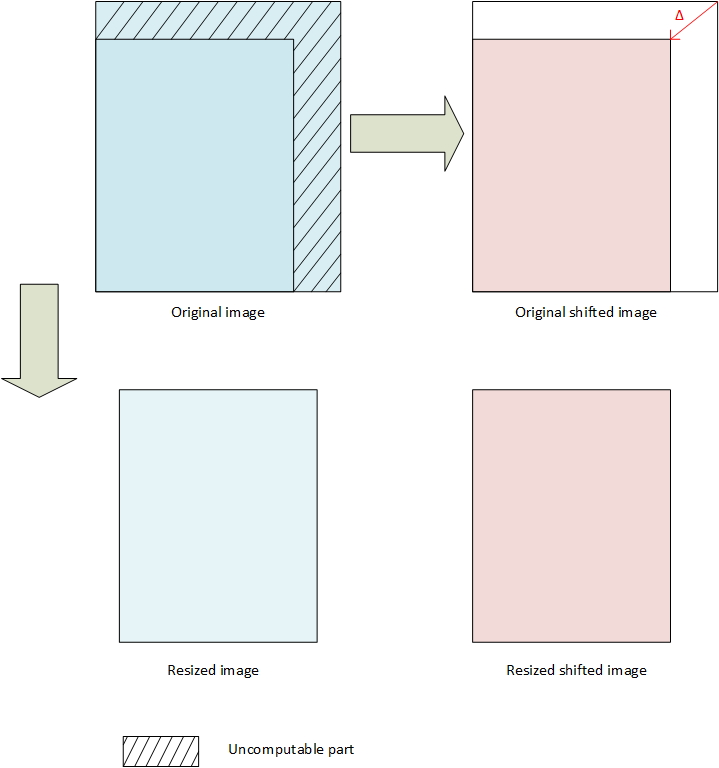
\includegraphics[scale=0.65]{ColorDiff.png}
    \caption{Color Difference illustration}\label{fig:Color Difference by image shifting illustration}
\end{figure}

To do that, the program will calculate the equivalent of the translation in horizontal and vertical pixel translation as show below .

\begin{figure}[h]
    \center
    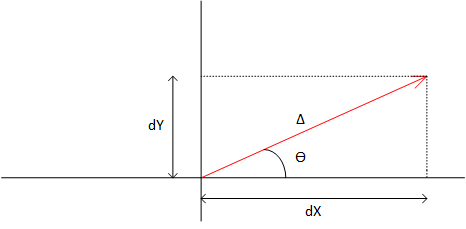
\includegraphics[scale=0.85]{illustrationVecteur.png}
    \caption{Vector to pixel distance}\label{fig:Vector to pixel distance}
\end{figure}

\begin{equation}
\begin{split}
&\sin\theta=dY/\|\Delta\| \\
&dY = \sin\theta * \|\Delta\| \\
&\cos\theta=dX/\|\Delta\| \\
&dX = \cos\theta * \|\Delta\|
\end{split}
\end{equation}

The values of $\|\Delta\|$ and $\theta$ have to being choose in the aim of get an entire number of pixel.

This computation gives us the C$_2$O matrix which corresponds to the cloud of point described in the State of art. To validate this part, we have to compare our results with theory. It's known that the L$^*$a$^*$b$^*$ space has different component :
\begin{itemize}
\item L$^*$ which is an achromatic component
\item a$^*$ which express the opposition between the red and the green
\item b$^*$ which express the opposition between the blue and the yellow
\end{itemize}


\begin{figure}[h]
    \center
    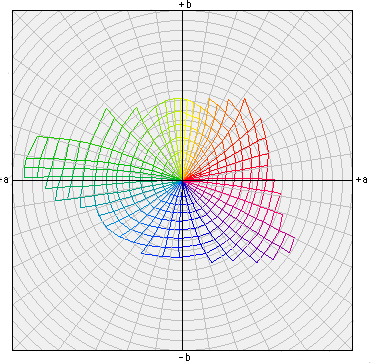
\includegraphics[scale=0.95]{BL_LAB.png}
    \caption{Lab space illustration}\label{fig:Lab space illustration}
\end{figure}
\newpage
We define two test images composed by a succession of line at different colors levels.

So if we are testing our program on images like the two one shown below which are containing the two same colors opposed on the same component of the  L$^*$a$^*$b$^*$ space, the result on the difference must show that :

\begin{itemize}
\item For the first one which is in green and red, there will be two points spaced on the a$^*$ component but at constant levels on the L$^*$ and the b$^*$ component.
\item For the second one which is in blue and yellow, there will be two points spaced on the b$^*$ component but at constant levels on the L$^*$ and the a$^*$ component.
\end{itemize}


\begin{figure}[h]
        \centering
        \begin{subfigure}[b]{0.5\textwidth}
                \centering
                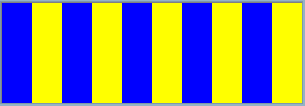
\includegraphics[height=70px]{TestIMG_BY.png}
        \end{subfigure}%
        \hfill
        \begin{subfigure}[b]{0.5\textwidth}
                \centering
                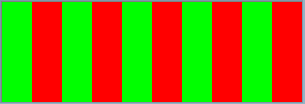
\includegraphics[height=70px]{TestIMG_RG.png}
        \end{subfigure}
        \caption{Test images}
        \label{fig:Test images}
\end{figure}

\begin{figure}[h]
        \centering
        \begin{subfigure}[b]{0.5\textwidth}
                \centering
                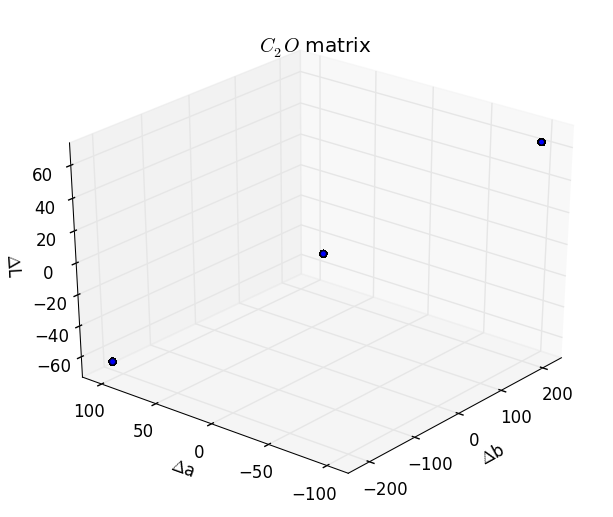
\includegraphics[height=220px]{MatriceC2O_ImgBleuJaune.png}
        \end{subfigure}%
        \hfill
        \begin{subfigure}[b]{0.5\textwidth}
                \centering
                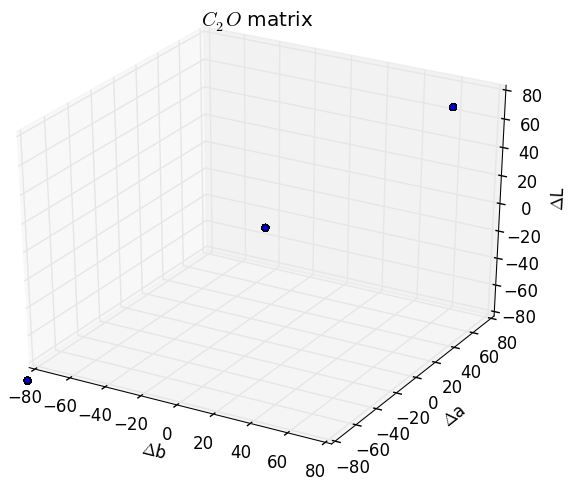
\includegraphics[height=220px]{MatriceC2O_ImgRougeVerte.png}
        \end{subfigure}
        \caption{Coorcurence matrix obtained from test images}
        \label{fig:Coorcurence matrix obtained from test images}
\end{figure}

With this step validate by the theory, we will have to test with more colors to verify that we obtain the right number of points on the coocurence matrix for the corresponding number of colors. For each test image, there will be more points as the number of colors on the image is growing because the number of difference of color will grow too.

\newpage
\subsection{The signature computing}

After doing that, we have to compute the spherical quantization of the probability matrix. For that, we have to transform our difference image from Carthesian coordinates to Spherical coordinates (from these one, the spherical quantization will be easier to compute). So we consider our Lab space like a 3 dimensional repository and for each points, it's calculate E the norm of the vector formed by the distance between it and the point (0,0,0), the orientation $\alpha$ formed by the angle between the vector and the a plan and finally the orientation $\beta$ formed by the angle between the vector and the b plan.


\begin{figure}[h]
    \center
    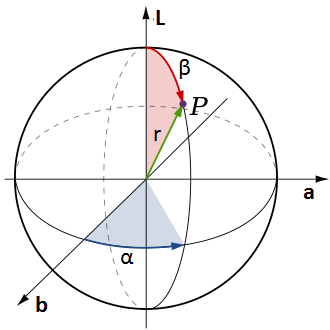
\includegraphics[scale=0.60]{Spherical_Coordinates.png}
    \caption{Spherical coordinates}\label{fig:Spherical coordinates}
\end{figure}

To calculate these coordinates, we have to use the following equations :

\begin{equation}
\begin{split}
&E = \sqrt{x^2+y^2+z^2} \\
&\alpha = \arctan(y/x) \\
&\beta = \arccos(z/r)
\end{split}
\end{equation}

So for each pixel we obtain :
\begin{itemize}
\item $\Delta$ E the color distance (approximately equivalent to the contrast)
\item $\Delta \alpha$ the orientation of the $\Lambda$ vector on the a, b plan (that give us an image of the hue)
\item $\Delta \beta$ the orientation of the $\Lambda$ vector on the L, b plan (that give us an image of the luminance)
\end{itemize}


In that way, we obtain our cloud of points in a spherical repository. Once we get it, we need to calculate our C2O signature by quantifying the cloud of point we obtain by a spherical quantization.


It's computed in three times :

There will we 4 interval of radius for the sphere :

\begin{equation}
\begin{split}
&0 \leq \Delta E < 3
\\&3 \leq \Delta E < 6
\\&6 \leq \Delta E < 9
\\&9 \leq \Delta E < infinite
\end{split}
\end{equation}


Each sphere will be split by $\alpha$ interval to concentrate the information as show below in the sectional view following the $(a^*,b^*)$ plan.
Each $\alpha$ interval will measure $\Delta\alpha=360/8$

This quantization has to be done for each value of $\beta$ interval which will measure $\Delta\beta=180/8$.

\begin{figure}[ht]
    \center
    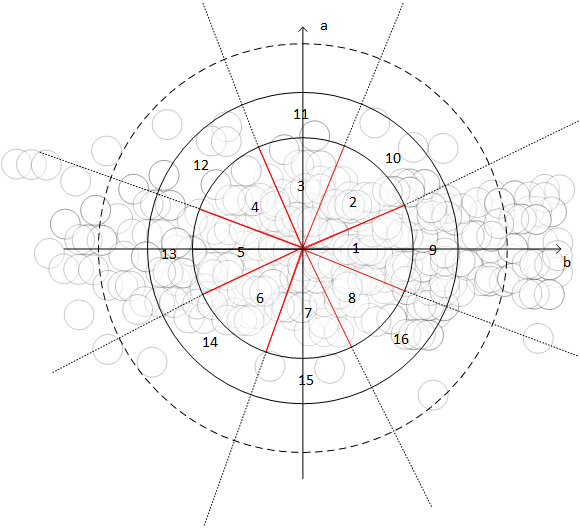
\includegraphics[scale=0.5]{QuantificationSphericToHist1.png}
    \caption{Spherical quantization following $\alpha$ and E}\label{fig:Qantification sph�rique}
\end{figure}


Once this quantization is done, the signature can be constituted by concatenate the values in a vector following a spiral for each value of $\beta$.

\begin{figure}[ht]
    \center
    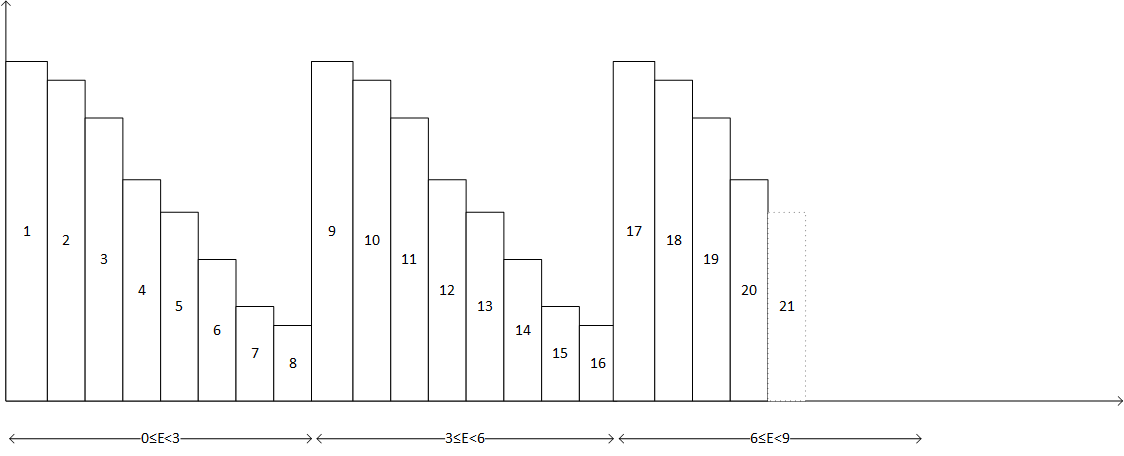
\includegraphics[scale=0.5]{QuantificationSphericToHist2.png}
    \caption{Spherical quantization following $\alpha$ and E}\label{fig:Qantification sph�rique}
\end{figure}

\newpage
The histograms obtained for each interval of $\beta$ will be concatenate to obtain the whole signature.

\begin{figure}[ht]
    \center
    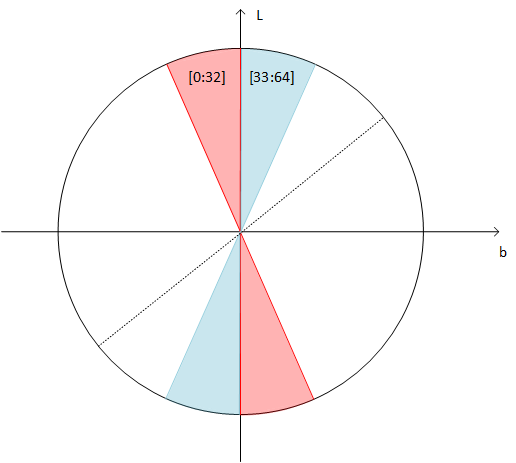
\includegraphics[scale=0.5]{QuantificationSphericToHist3.png}
    \caption{Spherical quantization following $\beta$ }\label{fig:Qantification sph�rique}
\end{figure}


\begin{figure}[ht]
    \center
    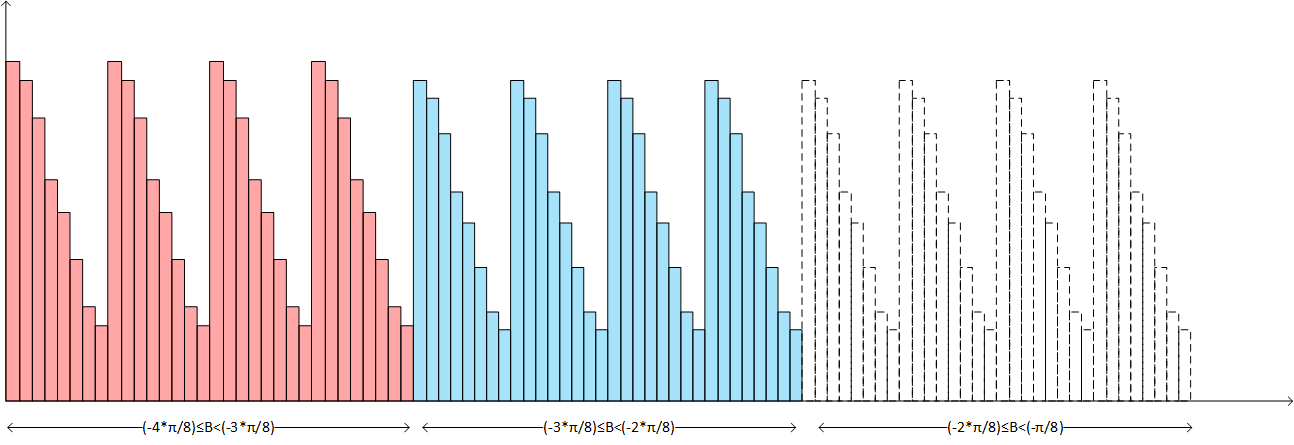
\includegraphics[scale=0.5]{QuantificationSphericToHist4.png}
    \caption{Spherical quantization following $\beta$}\label{fig:Qantification sph�rique}
\end{figure}



In this way, we obtain one unique vector of 256 values to describe the image.
\newpage
\subsection{Validation step}

Once these function are computed, the most important step is to validate the good operation of all the parts. So in this part we will firstly demonstrate the functioning of the transformation through the L$^*$a$^*$b$^*$ space, an after we will talk about the spherical quantization.
The functioning of the transformation in spherical coordinates will not been covered here because of the test to validate it is just making the inverse operation and verify is we get th same data..

\subsubsection{Validation of the transformation through L$^*$a$^*$b$^*$ space and color difference}

First of, we have to choose a reference to compare our results with. The solution choose is to compare the result of our function with those of the Bruce Lindbloom website's calculator which is a well know reference in image processing.

We has choose to work from the AdobeRGB space because it's one of the most used.
To compute correctly the L$^*$a$^*$b$^*$ space, we have to apply a $\gamma$ factor to make the operation called ��inverse companding��. This correction is made because we consider that the RGB space as it is capture by actual sensors is non linear because of the inequality of energy between low and hight luminosity levels.
The $\gamma$ inverse companding factor to apply is 2,2 and the standard illuminant is D65.
We can compare our results  with the Bruce Lindbloom website's calculator to verify that we obtain the good results.

Here we will make a first test with only 2 colors, the red and the green.
\vspace*{2mm}


\begin{equation}
\begin{split}
RGB =& [255 ,0 ,0] ~~/~~ L =61.4272~~  a=89.5619~~   b=75.1487
\\RGB =& [0 ,255 ,0] ~~/~~ L =83.3027~~  a=-137.9737~~   b=90.8299
\end{split}
\end{equation}

\vspace*{2mm}

Because of the construction of the image on which we are testing our program, there will be only to different values of color difference on each component so by calculate and compare it with the theoretical values, we could validate our color difference computation:
\vspace*{7mm}

$\Delta L_1$ = -21,8755
$\Delta a_1$ = 227,5356
$\Delta b_1$ = -15,6811

$\Delta L_2$ = 21,8755
$\Delta a_2$ = -227,5356
$\Delta b_2$ = 15,6811
\vspace*{7mm}

Here we will make a second test with Yellow and blue.
\vspace*{2mm}



\begin{equation}
\begin{split}
RGB& = [255 ,255 ,0] ~~/~~ L =97.0132~~  a=-22.5787 ~~  b=105.3055
\\RGB& = [0 ,0 ,255] ~~/~~ L =32.9786 ~~ a=80.3051 ~~  b=-109.3824
\end{split}
\end{equation}

\vspace*{2mm}
As it has been done for the first test, we will compare our result of color difference with the theoretical ones.
\vspace*{7mm}

$\Delta L_1$ = 64,0346
$\Delta a_1$ =  -102,8838
$\Delta b_1$ = 214,6879

$\Delta L_2$ = -64,0346
$\Delta a_2$ = 102,8838
$\Delta b_2$ = -214,6879
\vspace*{7mm}

These results are the same obtained with our program so we can consider that our Lab transformation and our color difference computation are valid.


\subsubsection{Validation of the spherical quantization}

Once we could be sure that our $C_2O$ matrix is the good one, we have to validate the operating of the spherical quantization which must extract the signature of the image from the $C_2O$ matrix.

For these tests, we will fix the number of intervals choose on each component : there are 4 intervals on $\Delta E$, 8 intervals on $\Delta \alpha$ and 8 intervals on $\Delta \beta$.
So we will obtain a signature of 256 values to describe the image. To validate our spherical quantization, we have to create a matrix in spherical coordinates in which we will fix all the values. The first test we will do is to fix our values to have all the points of our matrix in one only interval of $\alpha$. By doing that, we will be sure that the quantization is good because we will produce the values especially to be in one only interval of the final signature/histogram.

For example here we want to have all the values in the first interval of the histogram.

So the values of $\Delta E$ has to been fixed between 0 and 3, values of $\Delta \beta$ has to be between $\frac{-2 \pi }{16}$ and $\frac{2 \pi}{16}$ and the values of $\Delta \alpha$ has to be between  $\frac{-8 \pi }{16}$ and $\frac{-6 \pi }{16}$  (as show below)

\begin{figure}[H]
    \center
    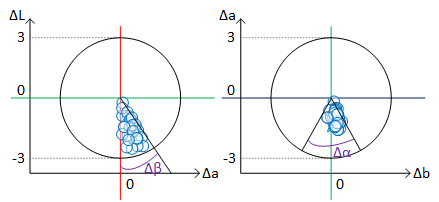
\includegraphics[scale=1]{IllustrationQuantifTheo.png}
    \caption{Quantization validation : point generation example}\label{fig:Illustration th quantif}
\end{figure}

So to do that, we generate these values by using a random function weighted by the right parameters and we obtain the following matrix�:

\begin{figure}[H]
    \center
    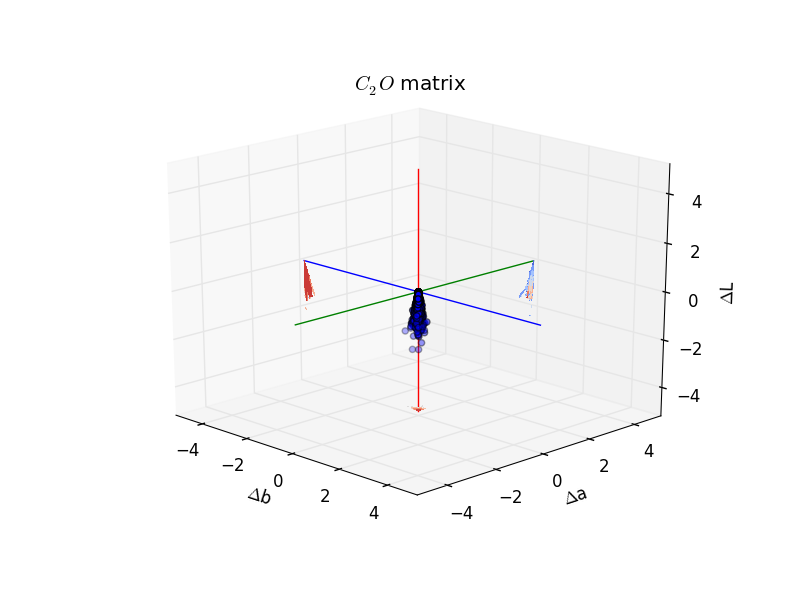
\includegraphics[scale=0.75]{QuantifInterv0.png}
    \caption{Quantization validation : point generation example}\label{fig:Illustration th quantif}
\end{figure}


Beginning with the same formulas, we are now able to write a general process to generate values in one only interval of the quantization following the calculation describe below�:
\vspace*{7mm}
\newline
$\Delta E$ = $\|(random(30,30))\|$*3 \newline
$\Delta E$ = $\Delta$ E + (3* NbInterE) \newline
$\Delta \alpha$ = $\|(random(30,30))\|$* $\frac{\pi}{8}$ \newline
$\Delta \alpha$ = $\Delta \alpha $+ $(NbInter \alpha * \frac {2* \pi}{8})$ \newline
$\Delta \beta$ =  $\|(random(30,30))\|$*$ \frac{\pi}{8}$ \newline
$\Delta \beta$ = $\Delta \beta$ � ((4-NbInter $\beta) * \frac {\pi}{8})$ \newline

For example, if we set  NbInterE to 0, $NbInter \alpha$ to 4 and  $NbInter \beta$ to 0, we must have all the 900 (30*30) values on the $4^th$ interval (8*4*0 + 8*0 + 4).

Here we can see the matrix that we obtain with these parameters�:


\begin{figure}[H]
    \center
    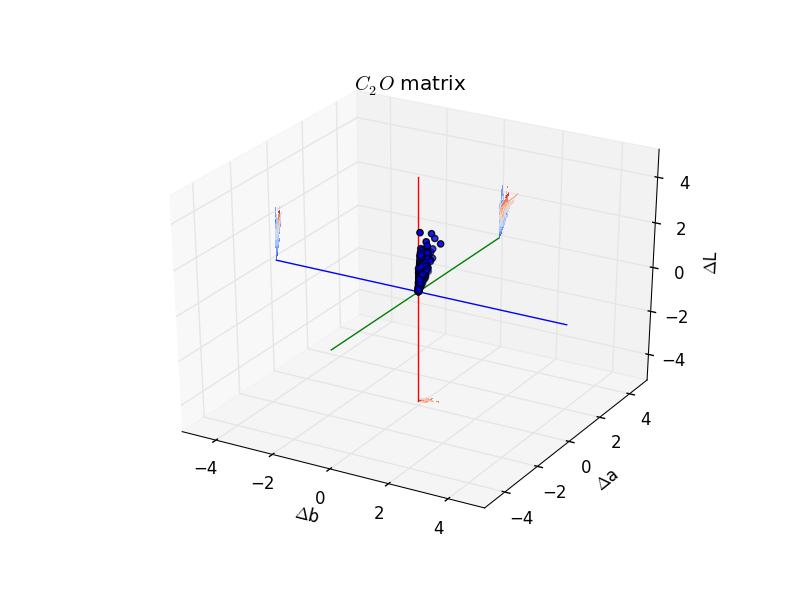
\includegraphics[scale=0.5]{MatC2OTestQuantifInterv4.png}
    \caption{C$_2$O matrix $4^{th}$ interval}\label{fig:Qantification sph�riquevalid1}
\end{figure}

So we have the following signature�:



\begin{figure}[H]
    \center
    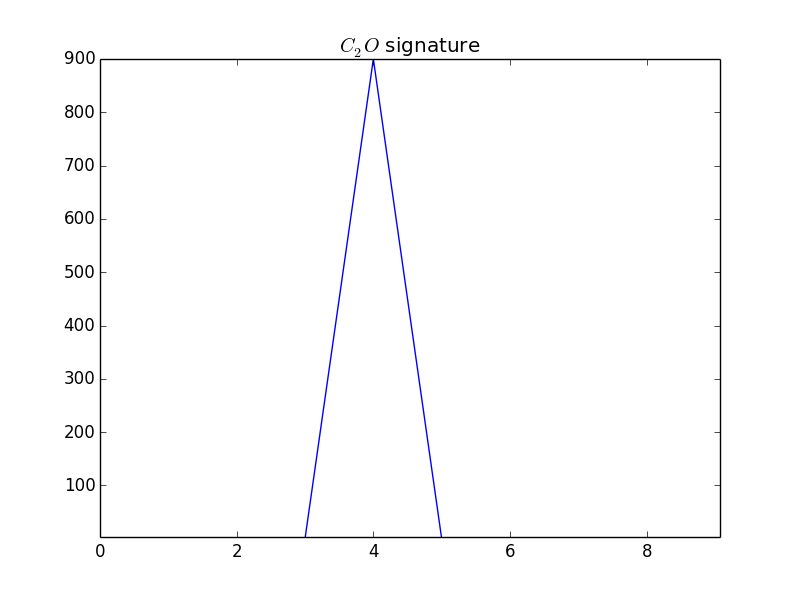
\includegraphics[scale=0.5]{SignatureTestQuantifInterv4.png}
    \caption{C$_2$O singnature $4^{th}$ interval}\label{fig:Qantification sph�riquevalid2}
\end{figure}

All the values are on the $4^{th}$ interval.

Let's test it for another interval. If we set NbInterE to 1, $NbInter \alpha$ to 3 and  $NbInter \beta$ to 1, we must have all the 900 (30*30) values on the $43^th$ interval (8*4*1 + 8*1 + 3).

The following matrix is obtained�:


\begin{figure}[H]
    \center
    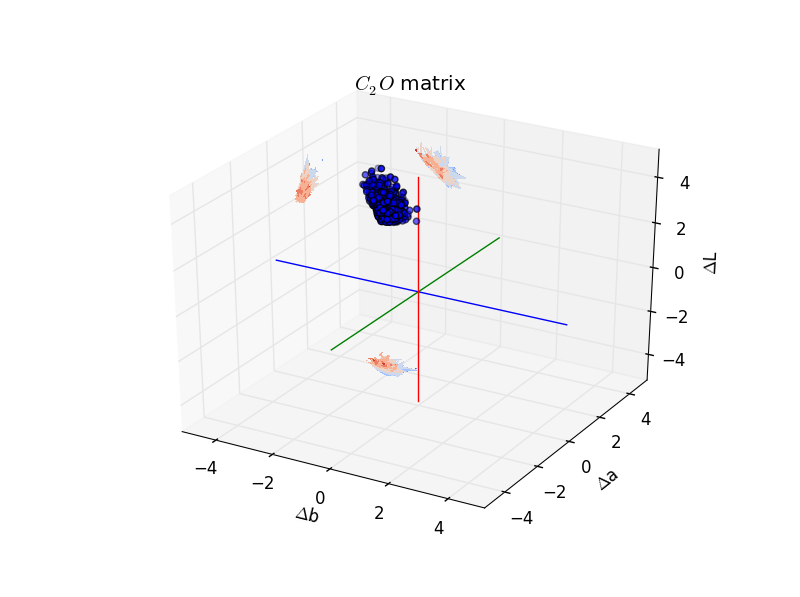
\includegraphics[scale=0.5]{MatC2OTestQuantifInterv43.png}
    \caption{C$_2$O matrix $43^{th}$ interval}\label{fig:Qantification sph�riquevalid3}
\end{figure}

So we obtain the following signature�:





\begin{figure}[H]
    \center
    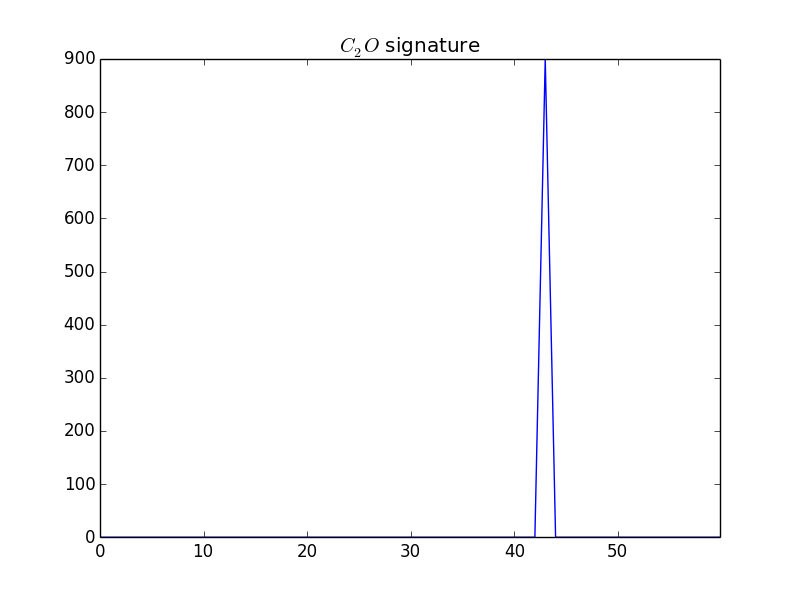
\includegraphics[scale=0.5]{SignatureTestQuantifInterv43.png}
    \caption{C$_2$O signature $43^{th}$ interval}\label{fig:Qantification sph�riquevalid4}
\end{figure}

All the values are on the $43^{th}$ interval.

Considering these results, we can validate operation of our spherical quantization.






% ----------------------------------------------------------------
\end{document} 